\documentclass[interim_report.tex]{subfiles}

\begin{document}

\section{Project Plan}
\subsection{Time Plan}
The given time plan outlined below provides me with a useful indication of how to measure the progress of the project, as well as dividing the whole project into smaller, more manageable sections which can be assessed individually. Some of the milestones have already been completed, while the others are expected to be finished within the given time period.
\subsubsection{Key Milestones}
\begin{itemize}
	\item Done - Background reading on DPDK \& Netmap
	\item Done - Understand workings off Java Native Interface (JNI) and Java memory
	\item Done - Get DPDK (and associated programs) working on local machine (or VM)
	\item In Progress - Link DPDK library with shared object files for JNI
	\item Awaiting - Implement basic IP address firewall
	\item Awaiting - Implement basic NAT
	\item Awaiting - Find similar implementations of firewall and NAT in C/C++ and Java
	\item Awaiting - Set up 2 independent machines to use for testing purposes
	\item Awaiting - Run tests on firewall and NAT to produces performance measurements
	\item Awaiting - Analyse results
\end{itemize}

\subsubsection{Time Estimations}
\begin{center}
	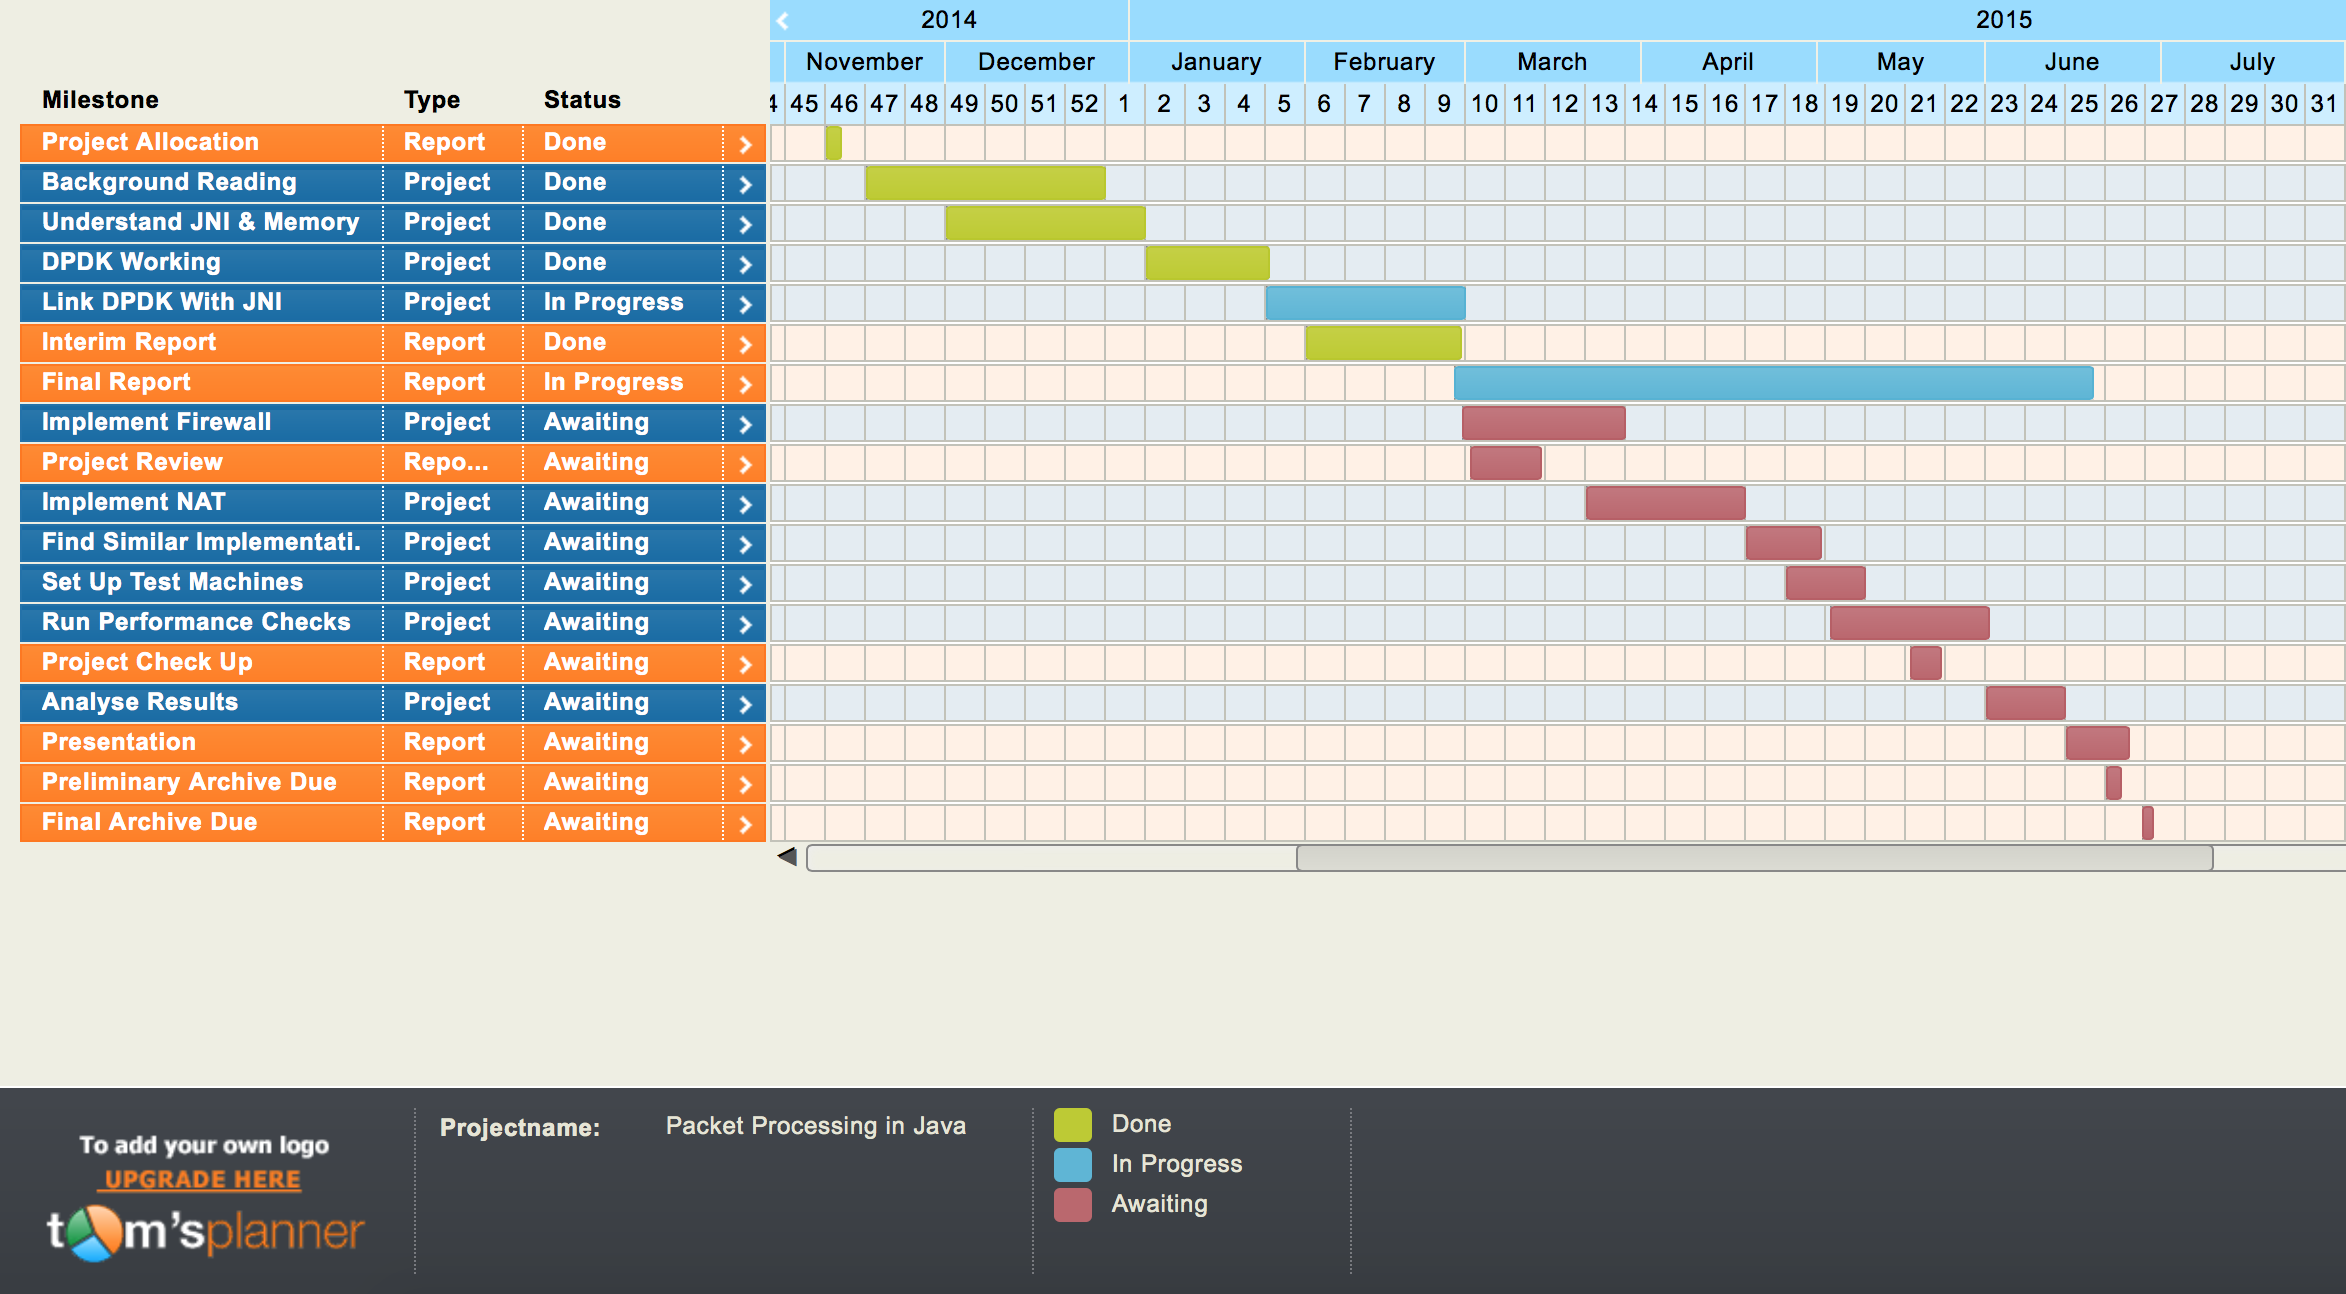
\includegraphics[width=\textwidth]{img/timeline.png}
\end{center}

\subsubsection{Completed Milestones}
As indicated, the background reading on the DPDK and Netmap libraries has been completed and analysis of existing code samples as been carried out in order to determine the usefulness of each of these libraries. As briefly mentioned in the Section~\ref{subsec:dpdk}, DPDK offers many benefits of using the library, including large existing documentation, very low latency for I/O operations and usability from Java applications via the JNI. This lead to the understanding off the JVM, JNI and memory access as it plays a vital part of the project, required in order to bypass certain features while exploiting others. \\
\newline
After basic research was carried out, the main task was to get DPDK working on a local machine so development wouldn't be restricted. The initial plan was to get it working straight on Mac OS X Yosemite, but after initial investigation this was deemed impossible due to the lack of NIC and operating system support. This lead to the creation of a virtual machine t (VM) running Ubuntu 14.04 LTS, which allowed for specific NIC's to be mimicked in order for DPDK to work correctly. This eventually led DPDK been built on the system and basic testing could be carried out to ensure all parts of the libraries were running correctly. The set-up stage was a long process due to lack of specific libraries existing from a fresh OS install and dependency issues. \\
\newline
Currently work on getting custom DPDK C files compiled into shared object files (.so) for use with the Java application is the main priority. Without this, the main idea for a solution to the initial objective isn't possible. Due to the complicated build process which DPDK uses in order to correctly access memory and libraries in the right order, generating the shared object file at the precise time is proving difficult. Work on this is still ongoing and is due to be completed within the near future.

\subsection{Fall Back Position}
If a number of unforeseen issues arise which impact on the progress of the project, I've outlined a few of the key milestones which can be omitted in order to allow the project to still be evaluated:
\begin{itemize}
	\item Implement basic NAT
	\item Find similar implementations of firewall and NAT in C/C++ and Java
	\item Run tests on firewall and NAT to produces performance measurements
\end{itemize}
Obviously, the emission of the above milestones will result in a less accurate evaluation of the overall project, but it's better than having nothing to evaluate in the end. As seen above, limiting the testing to one type of middlebox (only the firewall) can still give good results. This therefore reduces the need to look for an implementation for the NAT in Java and C/C++, while meaning less tests will have to be carried out. I feel that the remaining milestones are definitely key to the project in order for an adequate evaluation to be carried out.

\subsection{Possible Extensions}
If time allows, there are a number of possible extensions which can be undertaken to advance the project further forward and produce more data which can be evaluated later.

\subsubsection{Off Heap Java Memory}
In order for DPDK to handle packets correctly, it has to insert these packets onto the outgoing 'ring'. To do this, the Java application has to place its serialised objects into memory which DPDK can access. Under the current implementation, the Java application will directly place the packets onto the 'ring' using the direct ByteBuffer allocate feature. The other option is to use off heap java memory which DPDK can access and place onto the 'ring' automatically. This off heap memory is slightly slower than on heap memory but much faster than disk memory, while off heap memory stores object serialised and therefore ready for transmission in packets. \\
\newline
Altering the application to make use of off heap Java memory and then testing the results could potentially offer a new and faster way of high performance packet processing in Java.

\subsubsection{Limit Testing}
Another interesting extension could be to test the limitations of the NAT and firewall applications implemented within this project, and therefore limitations of the underlaying implementation. In terms of the project, the limitations could be on the max packet throughput which it can handle without having to buffer the incoming packets.

\end{document}